\documentclass[a4paper, 11pt]{article}
\usepackage[utf8]{inputenc}
\usepackage{authblk}
\usepackage{graphicx}
\usepackage{amsmath, amsfonts}
% NOTE: switched biblatex[style=ieee] -> natbib + bibtex (ieeetr) so the paper
% builds on Compute Canada (no biber / no biblatex core on the cvmfs TeX Live).
% Same IEEE numeric style; \cite{} is unchanged. Revert for an Overleaf build.
\usepackage[numbers,sort&compress]{natbib}
\usepackage{todonotes}
\usepackage{float}
\usepackage{hyperref}
\usepackage[margin=1in]{geometry}
\usepackage{subcaption}
\graphicspath{{mlcbCANDI_figs_png/}{Figures/}{./}}
\renewcommand{\thesubfigure}{\Alph{subfigure}}
\captionsetup{font=small}
\setlength{\textfloatsep}{3pt}\setlength{\abovecaptionskip}{3pt}
\setlength{\intextsep}{3pt}
\setlength{\floatsep}{3pt}

\setlength{\parindent}{0em}
\setlength{\parskip}{0.05em}
\renewcommand{\baselinestretch}{1}

\title{CANDI:\\ Self-Supervised and Confidence-Aware Denoising Imputation of Genomic Data}

\author[1]{\small Mehdi Foroozandeh}
\author[1]{Abdul Rahman Diab}
\author[1]{Maxwell Libbrecht}
\affil[1]{School of Computing Science, Simon Fraser University, Burnaby, Canada}
\date{}



\begin{document}

\maketitle

\section*{Abstract}
Large-scale epigenomic datasets such as histone modifications and DNA accessibility have greatly advanced our understanding of genomic function.  However, these measurements often suffer from noise, batch effects and irreproducibility. Epigenome imputation has emerged as a promising solution to these challenges. These methods integrate patterns across experiments, cell types, and genomic loci to predict the results of experiments, yielding predictions that often surpass observed data in quality. Thus, researchers increasingly leverage imputation for denoising data prior to downstream analysis. 

However, existing methods for imputation-based denoising have significant limitations. Here, we propose CANDI (Confidence-Aware Neural Denoising Imputer), a self-supervised deep learning method for epigenome imputation and denoising. CANDI takes as input raw read counts, DNA sequence, and experiment-specific covariates (e.g., sequencing depth and real length), and outputs three complementary predictions as probability distributions: raw counts (negative binomial), processed signal values (Gaussian), and peak calls (Bernoulli). CANDI can optionally incorporate information from a low-quality existing experiment when predicting a target without retraining. By conditioning on experimental metadata rather than learned cell-type embeddings, CANDI enables zero-shot generalization to unseen cell types without retraining. We demonstrate that CANDI achieves state-of-the-art performance in recovering epigenomic signal structure while providing calibrated uncertainty estimates.


% However, existing methods for imputation-based denoising have significant limitations. Here, we propose CANDI (Confidence-Aware Neural Denoising Imputer), a method for epigenome imputation that (1) gets as input raw counts and experiment-specific covariates such as sequencing depth,
% (2) can (optionally) incorporate information from a low-quality existing experiment when predicting a target without retraining, and (3) outputs a calibrated measure of uncertainty. This approach is enabled using self-supervised learning (SSL) training.


\section{Introduction}
    \input{introduction.tex}


% \newpage
\section{Results}\label{results}
    
\subsection{Self-supervised, confidence-aware denoising imputation of genomic data}

We propose CANDI, a method for imputation of the epigenome.

Briefly, CANDI works as follows (Section \ref{methods}) : For a given 30kb locus, CANDI takes as input:
\begin{enumerate}
    \item Observed epigenomic data sets (read counts) for the locus in the target sample along with the ChIP-seq control signal
    \item Four experimental covariates for each observed assay (sequencing depth, read length, run type, sequencing platform)
    \item The DNA sequence of the locus
\end{enumerate}

It also takes as input the experimental covariates of the desired outputs.

CANDI outputs predicted epigenomic data sets for the given locus and sample in three formats:
\begin{enumerate}
    \item \textbf{Raw read counts} as a negative binomial distribution per genomic position per assay
    \item \textbf{Continuous signal} in $\operatorname{arcsinh}\left(\text{signal p-value}\right)$ units as a Gaussian distribution per genomic position per assay
    \item \textbf{Peak calls} as binary classification probabilities per genomic position per assay
\end{enumerate}


All outputs are given in the form of probability distributions, enabling calibrated uncertainty quantification.

CANDI consists of a neural network model that includes convolutional, self-attention and deconvolutional layers with per-layer metadata cross-attention (Figure \ref{fig:architecture}). We trained CANDI using a self-supervised learning approach by optimizing three complementary objectives:
\begin{enumerate}
    \item \textbf{Full assay masking}: We mask entire assays and ask CANDI to predict these masked assays from the remaining available ones (mimicking imputation).
    \item \textbf{Full loci masking}: We mask the same genomic positions across all assays and ask CANDI to predict these masked positions (mimicking masked language modeling \cite{ji2021dnabert, devlin2019bert}).
    \item \textbf{Denoising via downsampling}: We simulated low-quality data by downsampling reads from training tracks and asked CANDI to predict the original high-depth data from low-quality observations (mimicking denoising).
\end{enumerate}

\begin{figure}[tbp]
    \centering
    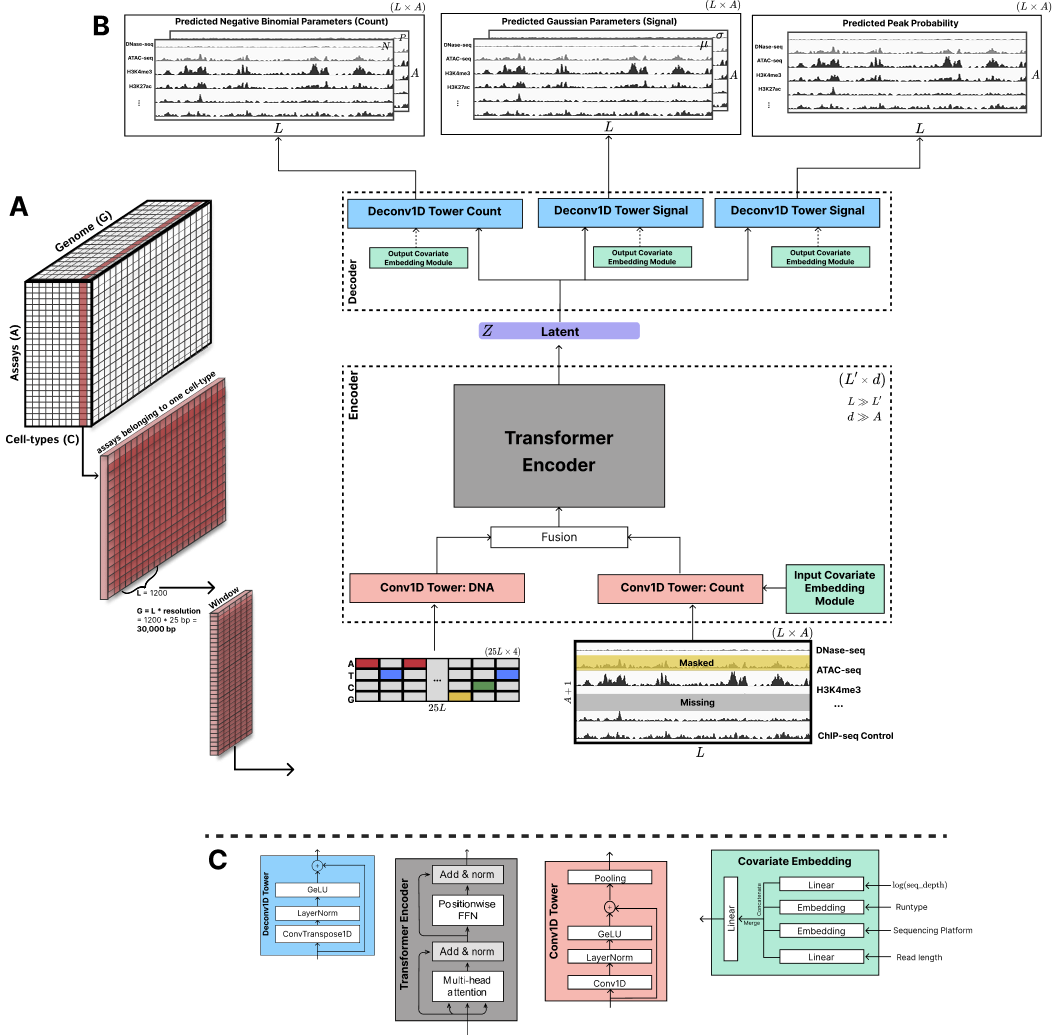
\includegraphics[width=0.66\textwidth]{fig1_architecture}
    \caption{\textbf{CANDI architecture overview.} (A) Input data organization showing the three-dimensional structure of epigenomic data across assays, genomic positions, and cell types. (B) Model architecture consisting of encoder and decoder components. The encoder processes DNA sequence and epigenomic count data through parallel convolution towers with per-layer metadata cross-attention, integrates experimental covariate information, and generates a latent representation using a transformer encoder with rotary positional embeddings. Three separate decoders predict count data (negative binomial parameters), signal values (Gaussian parameters), and peak locations (binary classification) for each assay and position. (C) Detailed architecture of key model components including convolution and deconvolution towers, transformer encoder blocks, and the metadata embedding module.}
    \label{fig:architecture}
\end{figure}

\subsection{CANDI accurately imputes missing epigenetic signals}
We first assessed CANDI's ability to accurately impute missing epigenomic signals across diverse cell types and experimental assays, evaluated genome-wide across a wide range of epigenetic marks and cell types.

We benchmarked CANDI on the ENCODE Imputation Challenge (EIC) dataset \cite{schreiber2023encode}, a standardized benchmark for evaluating epigenomic imputation methods. We compared CANDI-predicted signals with the following baseline and challenge-winning methods: (1) average (naive baseline), (2) Avocado \cite{schreiber2020avocado}, (3) Guacamole, (4) Lavawizard, (5) imp (an early version of eDICE \cite{hawkins2023getting} that participated in EIC), and (6) Hongyang Li and Yuanfang Guan v1. For this comparison, we followed the train-test split of the EIC dataset. To avoid memorization bias, especially regarding DNA sequences, we excluded chromosome 21 from the CANDI training dataset and tested exclusively on this chromosome.

In terms of global genome-wide correlation, CANDI significantly outperforms all EIC competitors in Spearman correlation across all assays (Figure \ref{fig:imp}: A). However, it under-performs in Pearson correlation for most assays  (Figure \ref{fig:imp}: B). This discrepancy highlights a key characteristic of the model: while CANDI is highly effective at recovering the correct rank-ordering and structural patterns of epigenomic signals (high Spearman), it tends to underestimate the absolute magnitude of high-signal regions (lower Pearson). This is evident in the scatter density plots, where predicted values in $\text{arcsinh}$ space show strong monotonic correlation with observations but a compressed dynamic range (Figure \ref{fig:imp}: C, D). Comparing against the `Quantile Normalized' and `Reprocessed' baselines of the EIC, which attempt to correct for train-test covariate shifts, further confirms that CANDI's structural imputation is state-of-the-art, even if signal magnitude scaling remains a challenge.

Unlike other methods, CANDI performs imputation solely based on the combinatorial patterns of the available assays in a given cell type; it receives no explicit cell type or positional information, requiring the model to infer generalizable patterns rather than memorizing position- or cell type-specific signals. This design choice presents a more challenging problem than methods that explicitly leverage cell type or positional metadata, but it enables efficient zero-shot imputation on new cell types using patterns learned during self-supervised pretraining.

Beyond correlation, we assessed prediction quality using peak classification metrics (Figure \ref{fig:imp}: E, F). CANDI demonstrates very high performance in distinguishing signal from background, achieving near-perfect AUROC ($\sim$1.0) for marks like H3K4me3, even where Pearson correlation was moderate ($\sim$0.35). This suggests that while exact signal values may be compressed, the biological signal-to-noise ratio is preserved, allowing accurate peak calling.

% While our benchmark comparisons followed the exact train-test split of the EIC dataset (Figure 2D, E), we adopted a different strategy for the extended dataset to simulate the more challenging cell type-agnostic scenario (Figure 2A,B,C). In the EIC train-test split, a subset of assays within a given cell type is reserved for testing or validation. For example, from 10 available assays in a given cell type, 7 may be used for training, and 3 reserved for testing. This approach assumes cell type-specific embeddings, where models must know the cell type at test time to impute the reserved assays. In contrast, our approach reserves entire cell types for training, testing, and validation. This ensures that at test time, the model encounters completely new cell types with only a few available assays, better mimicking real-world imputation. By doing so, we enforce a cell type-agnostic framework, requiring CANDI to generalize across unseen cell types based solely on learned patterns.


\begin{figure}[tbp]
    \centering
    \begin{subfigure}[b]{0.70\textwidth}\centering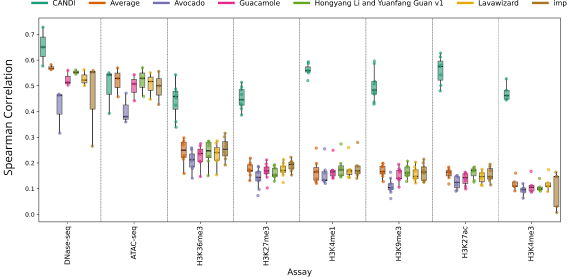
\includegraphics[width=\linewidth]{imp_spearman}\caption{}\end{subfigure}

    \begin{subfigure}[b]{0.70\textwidth}\centering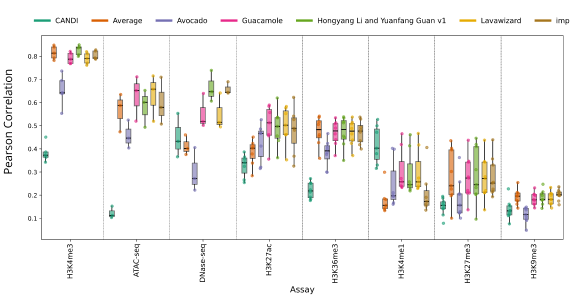
\includegraphics[width=\linewidth]{imp_pearson}\caption{}\end{subfigure}

    \begin{subfigure}[b]{0.28\textwidth}\centering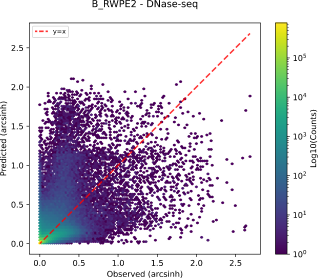
\includegraphics[width=\linewidth]{imp_scatter_dnase}\caption{}\end{subfigure}\hfill
    \begin{subfigure}[b]{0.28\textwidth}\centering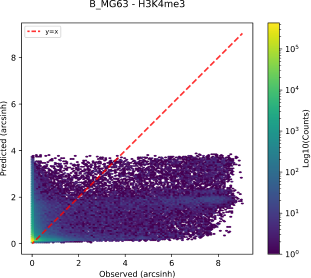
\includegraphics[width=\linewidth]{imp_scatter_h3k4me3}\caption{}\end{subfigure}\hfill
    \begin{subfigure}[b]{0.205\textwidth}\centering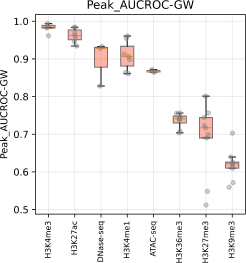
\includegraphics[width=\linewidth]{imp_peak_auroc_gw}\caption{}\end{subfigure}\hfill
    \begin{subfigure}[b]{0.205\textwidth}\centering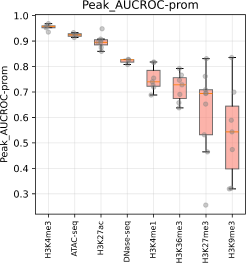
\includegraphics[width=\linewidth]{imp_peak_auroc_prom}\caption{}\end{subfigure}
    \caption{\textbf{Evaluation of CANDI imputation performance.} \textbf{(A)} Box plots displaying the genome-wide Spearman correlation coefficients for CANDI (teal) compared to baseline and top-performing EIC methods across various epigenetic assays. CANDI demonstrates superior performance in recovering signal rank-ordering. \textbf{(B)} Genome-wide Pearson correlation coefficients across assays. CANDI generally exhibits lower Pearson correlations compared to competitors, reflecting an underestimation of absolute signal magnitudes. \textbf{(C, D)} Scatter density plots comparing observed versus CANDI-predicted signal values (transformed to arcsinh space) for \textbf{(C)} DNase-seq in B\_RWPE2 cells and \textbf{(D)} H3K4me3 in B\_MG63 cells. The red dashed line indicates $y=x$. While the predictions show strong monotonic trends, the dynamic range is compressed relative to observations. \textbf{(E, F)} Peak classification performance assessed by the Area Under the Receiver Operating Characteristic (AUROC) curve for \textbf{(E)} genome-wide (Peak\_AUCROC-GW) and \textbf{(F)} promoter regions (Peak\_AUCROC-prom). CANDI achieves high classification accuracy across most marks, particularly for H3K4me3.}
\label{fig:imp}
\end{figure}


\subsection{CANDI provides calibrated aleatoric uncertainty estimates}

A core innovation of CANDI is its ability to output probability distributions rather than point estimates, providing a measure of uncertainty. Specifically, it captures aleatoric uncertainty, the uncertainty caused by the inherent randomness in experimental data due to biological variation, technical noise, and experimental biases.  Standard evaluation metrics like MSE or correlation collapse these distributions into their means, discarding valuable information about what the model ``knows it doesn't know.'' For each prediction, CANDI allows generating confidence intervals around the predicted distribution's mean enabling soft prediction of observed signals i.e. even if the observed value does not exactly match the mean of the predicted distribution, it falls within a predicted confidence interval.

We evaluated the fidelity of these uncertainty estimates using confidence calibration curves. A perfectly calibrated model would show a 1:1 relationship between the predicted confidence interval (e.g., 95\%) and the empirical coverage (the fraction of observed data points falling within that interval). We observed that calibration varies by assay type; chromatin accessibility assays (like DNase-seq) generally show better calibration than histone modifications (Figure \ref{fig:conf}: C, D). Typically, the model tends to be overconfident at lower confidence intervals ($c<0.5$) but becomes more calibrated and reliable at practically relevant intervals (0.9--0.95).

To further quantify the quality of these distributions, we utilized the Concordance Index (C-index), which evaluates whether the predicted distributions correctly rank-order the data while accounting for uncertainty. Genome-wide C-index scores were generally high. While H3K4me3 showed a lower genome-wide C-index ($\sim$0.6), its performance increases to $\sim$0.83 in promoter regions, where the mark is enriched  (Figure \ref{fig:conf}: A, B).

Visualizing the predicted Coefficient of Variation ($\text{CV} = \sigma/\mu$) reveals that CANDI assigns higher uncertainty to regions where it predicts low signal but the ground truth might be high  (Supplementary Figure~\ref{fig:cv}). In these ``missed'' regions, the model effectively flags its own potential error by outputting high variance, a capability absent in deterministic MSE-trained models.



\begin{figure}[tbp]
    \centering
    \begin{subfigure}[b]{0.235\textwidth}\centering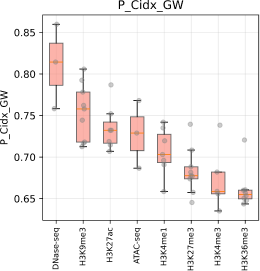
\includegraphics[width=\linewidth]{unc_cindex_gw}\caption{}\end{subfigure}\hfill
    \begin{subfigure}[b]{0.235\textwidth}\centering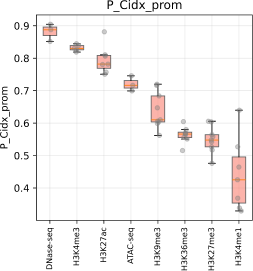
\includegraphics[width=\linewidth]{unc_cindex_prom}\caption{}\end{subfigure}\hfill
    \begin{subfigure}[b]{0.235\textwidth}\centering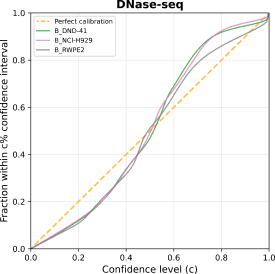
\includegraphics[width=\linewidth]{unc_calib_dnase}\caption{}\end{subfigure}\hfill
    \begin{subfigure}[b]{0.235\textwidth}\centering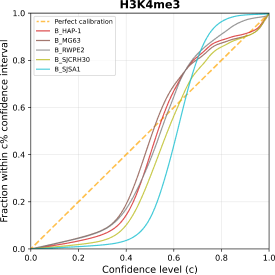
\includegraphics[width=\linewidth]{unc_calib_h3k4me3}\caption{}\end{subfigure}

    \begin{subfigure}[b]{0.28\textwidth}\centering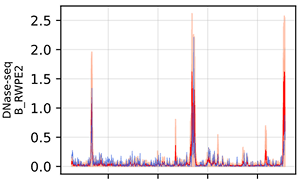
\includegraphics[width=\linewidth]{unc_track_dnase}\\ {\scriptsize Genomic position}\caption{}\end{subfigure}\hfill
    \begin{subfigure}[b]{0.28\textwidth}\centering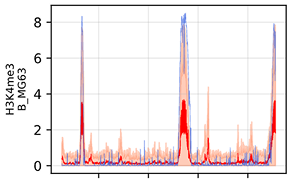
\includegraphics[width=\linewidth]{unc_track_h3k4me3}\\ {\scriptsize Genomic position}\caption{}\end{subfigure}
        \caption{\textbf{Evaluation of CANDI’s uncertainty estimation.}
        \textbf{(A, B)} Box plots showing the Concordance Index (C-index), a metric evaluating the quality of the predicted probability distributions, for \textbf{(A)} genome-wide regions and \textbf{(B)} promoter regions. While genome-wide scores vary, calibration improves significantly in signal-enriched promoter regions (e.g., H3K4me3).
        \textbf{(C, D)} Confidence calibration curves for \textbf{(C)} DNase-seq and \textbf{(D)} H3K4me3 across multiple cell lines. The plots compare the predicted confidence level ($c$) against the actual fraction of data falling within that interval. The dashed orange line represents perfect calibration; CANDI shows stronger calibration for accessibility assays compared to histone marks.
        \textbf{(E, F)} Representative genomic signal tracks for \textbf{(E)} DNase-seq and \textbf{(F)} H3K4me3. The blue line represents the observed signal, while the red line and shading represent the CANDI predicted mean and confidence intervals, demonstrating how the model captures signal within its uncertainty bounds.}
    \label{fig:conf}
    \end{figure}


\subsection{CANDI  imputed signals and latent space predict gene expression}

To validate the biological utility of CANDI's predictions, we assessed whether they could predict gene expression levels from RNA-seq data (in $\log(\text{TPM} + 1)$ units) better than raw data. We extracted features from transcription start site (TSS), gene body, and transcription end site (TES) using four sources: (1) Observed signals (available assays), (2) Denoised signals (available assays), (3) Denoised + Imputed signals (all 35 assays), and (4) CANDI's Latent Embeddings ($\mathbf{Z}$).

Our results show that denoised signals marginally outperform raw observed signals, indicating that CANDI successfully removes noise while preserving regulatory information. More importantly, the full set of 35 denoised and imputed assays outperforms the subset of available denoised assays, confirming that the imputation process adds meaningful regulatory context missing from the sparse input. Most strikingly, the best predictive performance was achieved using CANDI's latent embeddings ($\mathbf{Z}$) (Figure \ref{fig:biol}: A). This suggests that the latent space encodes rich, biologically relevant information---possibly higher-order regulatory logic or chromatin states---that is not fully captured when decoded back into low-dimensional signal tracks.

Furthermore, while the predictive power of observed and denoised signals depends heavily on the number of available input assays, the performance of the Imputed+Denoised and Latent settings is robust to input sparsity, demonstrating CANDI's ability to compensate for missing data (Figure \ref{fig:biol}: B).

\subsection{CANDI-derived chromatin state annotations are more reproducible}

A primary downstream use of epigenomic data is chromatin state annotation, yet these annotations are notoriously irreproducible when derived from noisy or sparse measurements~\cite{shahraki2024robust}. Because CANDI denoises and imputes epigenomic signal while explicitly modeling its uncertainty, we hypothesized that annotations built on CANDI's outputs would be more reproducible than those built on observed data. We annotated six held-out biosamples with an 18-state hidden Markov model using four input sources---observed signals, CANDI denoised signals, CANDI denoised+imputed signals, and CANDI latent embeddings---and measured reproducibility using SAGAconf's robustness ratio, the fraction of the genome assigned a confident, reproducible chromatin state (Methods).

In every biosample, at least one CANDI-derived source yielded a more reproducible annotation than observed data, and the latent representation $\mathbf{Z}$ was the most consistently reproducible, achieving the highest robustness ratio in four of the six biosamples (Figure~\ref{fig:biol}C shows two representative biosamples; all six in Supplementary Figure~\ref{fig:saga_full}). The improvement was often substantial: in neural progenitor cells, the latent-derived annotation confidently reproduced 87\% of the genome compared to 60\% for observed data. This parallels our gene-expression results---the same denoised, imputed, and latent representations that best predict transcription also produce the most reproducible chromatin state annotations---indicating that CANDI distills consistent biological structure from noisy measurements rather than merely smoothing the input signal.

\begin{figure}[tbp]
    \centering
    \begin{subfigure}[b]{0.27\textwidth}\centering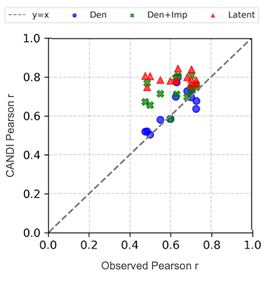
\includegraphics[width=\linewidth]{rna_scatter}\caption{}\end{subfigure}\hspace{0.03\textwidth}%
    \begin{subfigure}[b]{0.42\textwidth}\centering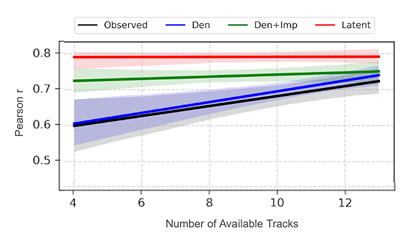
\includegraphics[width=\linewidth]{rna_vs_ntracks}\caption{}\end{subfigure}

    \begin{subfigure}[b]{0.78\textwidth}\centering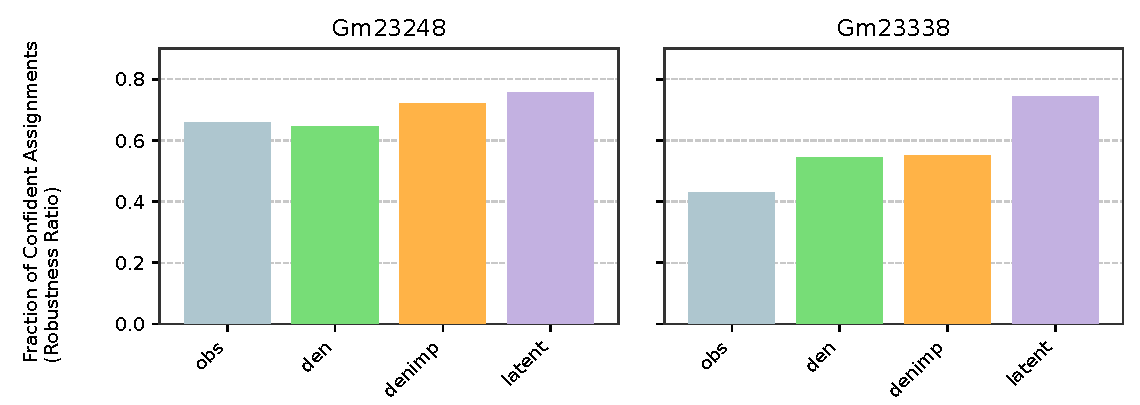
\includegraphics[width=\linewidth]{saga_top2.pdf}\caption{}\end{subfigure}
    \caption{\textbf{CANDI-derived features support downstream biological analyses.}
    \textbf{(A)} Scatter plot comparing gene expression prediction performance (Pearson correlation) using features derived from observed data ($x$-axis) versus CANDI-derived features ($y$-axis). CANDI's Latent embeddings (red triangles) consistently yield the highest predictive accuracy, outperforming Denoised (blue circles) and Denoised+Imputed (green crosses) inputs.
    \textbf{(B)} Line plot showing gene expression prediction performance as a function of the number of available input tracks. The performance of Latent embeddings (red) and Imputed signals (green) is robust to data sparsity, whereas the predictive power of Observed (black) and Denoised (blue) features declines with fewer input tracks.
    \textbf{(C)} Chromatin state annotation reproducibility for two representative held-out biosamples. Bars show the SAGAconf robustness ratio (the fraction of the genome receiving a confident, reproducible state assignment; higher is more reproducible) for annotations built from four input sources---observed signals (\emph{obs}), CANDI denoised signals (\emph{den}), CANDI denoised+imputed signals (\emph{denimp}), and CANDI latent embeddings (\emph{latent}). All six biosamples are shown in Supplementary Figure~\ref{fig:saga_full}.}
    \label{fig:biol}
\end{figure}




% \section{Discussion}
% Effective denoising imputation with CANDI promises to greatly improve all downstream applications of epigenomic data sets, including chromatin state annotation and predictive modeling. 
% CANDI enables the creation of ``supertracks'' that simulate a complete data set with excellent experiment quality and uniform experimental parameters. 

% \todo[inline]{
% 
% 
% Future work: 
% This can make supertracks; evaluating them is future work. 
% Train/evaluate across replicates. 
%Future work: evaluate latent representation. 
% 
%Maybe there is a better way of masking features? 
% 
% This confirms the hypothesis that it's possible to do imputation while being CT-agnostic and position-agnostic.
% Epistemic vs aleatoric uncertainty. Epistemic uncertainty is reducible but aleotoric is not: even replicates of the same experiment are not exactly the same. 
% }

% \newpage
\section{Methods}
    % methods.tex
% CANDI: Confidence-Aware Neural Denoising Imputer for Epigenomic Data
\label{methods}
\subsection{Data}

We trained and evaluated CANDI using two datasets. We used data from the ENCODE Imputation Challenge (EIC) \cite{schreiber2023encode}, featuring 35 distinct assays measured across 50 biosamples, following the original EIC train-validation-test split; since CANDI uses read counts as input, we obtained the corresponding raw read files (BAM). To have a more extensive dataset, we systematically collected data for all biosamples in the ENCODE database that contained at least one experiment from the 35 assays of interest, yielding 3,064 biosamples that we merged using a cell type-based merging strategy into a final dataset of 361 merged cell types. For each biosample containing ChIP-seq experiments, we include the corresponding ChIP-seq control as an additional always-available input channel that is never masked, and we simulate varying sequencing depths by read downsampling (Downsampling Factor $\in \{1, 2, 4\}$). Full data collection and processing details are in Supplementary Methods.

\subsection{CANDI Architecture}

Let $A = 35$ be the number of assays and $L = 1{,}200$ the number of 25 bp positions in a $G = 30{,}000$ bp window. For each cell type, CANDI receives the epigenomic read-count matrix $\mathbf{M} \in \mathbb{R}^{N \times L \times (A+1)}$ (the $(A{+}1)$-th channel is the always-available ChIP-seq control), the one-hot DNA sequence $\mathbf{S} \in \{0,1\}^{N \times 4 \times G}$, and input and output experimental covariates $\mathbf{C}_{\text{in}}, \mathbf{C}_{\text{out}}$ (four per assay: $\log_2$ sequencing depth, run type, read length, and sequencing platform). Input counts are transformed using $\text{arcsinh}(x)$ before the encoder, which stabilizes variance across the dynamic range of read counts.

An encoder $\mathcal{E}$ maps $(\mathbf{M}, \mathbf{S}, \mathbf{C}_{\text{in}})$ to a latent representation $\mathbf{Z}$ through parallel convolution towers with per-layer MetadataCrossAttention that conditions features on covariates using FiLM (Feature-wise Linear Modulation) \cite{perez2018film}, a fusion layer, and $n_{\text{sab}} = 4$ transformer encoder layers ($n_{\text{head}} = 9$) with rotary positional embeddings (RoPE). For each assay $a$ and position $\ell$, three separate deconvolution decoders---each conditioned on the output covariates $\mathbf{C}_{\text{out}}$---predict the parameters of a negative binomial $(\hat{n}_{a,\ell}, \hat{p}_{a,\ell})$ over raw counts, a Gaussian $(\hat{\mu}_{a,\ell}, \hat{\sigma}^2_{a,\ell})$ over $\text{arcsinh}$-transformed signal $p$-values, and a peak probability $\text{peak}_{a,\ell} \in [0,1]$. The negative binomial captures the overdispersion of sequencing counts, and the predicted Gaussian variance captures position-varying (aleatoric) uncertainty (Supplementary Methods).

\subsection{Learning Objectives and Training Strategy}

Our approach leverages self-supervised learning, where the model learns to reconstruct deliberately corrupted versions of its own input, by combining three complementary strategies (Section \ref{results}): full assay masking (mimicking imputation), full loci masking (mimicking masked language modeling), and denoising via downsampling. We train CANDI by minimizing $\mathcal{L} = w_{\text{obs}}\, \mathcal{L}_{\text{obs}} + w_{\text{imp}}\, \mathcal{L}_{\text{imp}}$, where each of $\mathcal{L}_{\text{obs}}$ (unmasked positions) and $\mathcal{L}_{\text{imp}}$ (masked positions) is a weighted sum of the negative binomial (count), Gaussian (signal), and binary cross-entropy (peak) negative log-likelihoods, with default weights $w_{\text{count}} = 0.5$, $w_{\text{pval}} = 1.0$, $w_{\text{peak}} = 0.1$, $w_{\text{obs}} = 0.25$, and $w_{\text{imp}} = 1.0$. We trained CANDI on 5,000 selected, non-overlapping 30kb regions, excluding chromosome 21 and reserving it exclusively for testing (Supplementary Methods).

\subsection{Evaluation Metrics}

To evaluate imputation performance, we compute genome-wide Mean Squared Error (MSE), Pearson correlation, and Spearman correlation; all performance evaluations were made on chromosome 21. For peak prediction, we evaluate using precision, recall, and area under the ROC curve (AUROC) against ENCODE narrowPeak calls. To assess the reliability of the model's uncertainty estimates, we measure calibration---the fraction of observed values that fall within the model's predicted $C\%$ confidence interval---and the Concordance Index (C-index), which assesses whether the predicted distributions correctly rank-order the data while accounting for uncertainty (Supplementary Methods). As biological validation, we evaluate how well epigenomic features derived from the model's predictions---from observed, denoised, denoised+imputed, and latent ($\mathbf{Z}$) sources---predict gene expression levels (RNA-seq $\log(\text{TPM}+1)$) via nested cross-validation. We further assess whether CANDI improves the reproducibility of downstream chromatin state annotation: for each source we annotate the genome with an 18-state HMM (a soft-evidence HMM for CANDI's Gaussian predictions, so that predictive uncertainty propagates into the annotation) and quantify reproducibility with SAGAconf's robustness ratio~\cite{shahraki2024robust} (Supplementary Methods).


\noindent\textbf{Data and Code Availability.} All codes, implementation details, and data collection procedures are available at \url{https://github.com/mehdiforoozandeh/CANDI}.

\bibliographystyle{ieeetr}
\bibliography{main}

\newpage
\appendix
% supplement.tex — Supplementary material for CANDI (MLCB submission)
% The main paper is self-contained; this appendix provides extended methods and figures.

\setcounter{figure}{0}
\renewcommand{\thefigure}{S\arabic{figure}}

\section{Supplementary Figures}

\begin{figure}[H]
    \centering
    \begin{subfigure}[b]{0.42\textwidth}\centering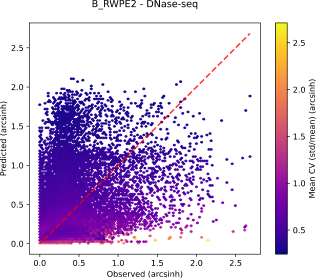
\includegraphics[width=\linewidth]{unc_cv_dnase}\caption{}\end{subfigure}\hfill
    \begin{subfigure}[b]{0.42\textwidth}\centering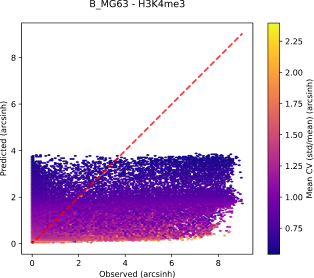
\includegraphics[width=\linewidth]{unc_cv_h3k4me3}\caption{}\end{subfigure}
    \caption{\textbf{Predicted coefficient of variation flags under-predicted signal.} Scatter density plots of predicted vs.\ observed signals (in $\text{arcsinh}$ space) colored by the predicted Coefficient of Variation (CV) for \textbf{(A)} DNase-seq and \textbf{(B)} H3K4me3. High CV values (yellow/orange) in regions where the model under-predicts signal magnitude indicate that CANDI correctly assigns high aleatoric uncertainty to these predictions.}
    \label{fig:cv}
\end{figure}

\begin{figure}[H]
    \centering
    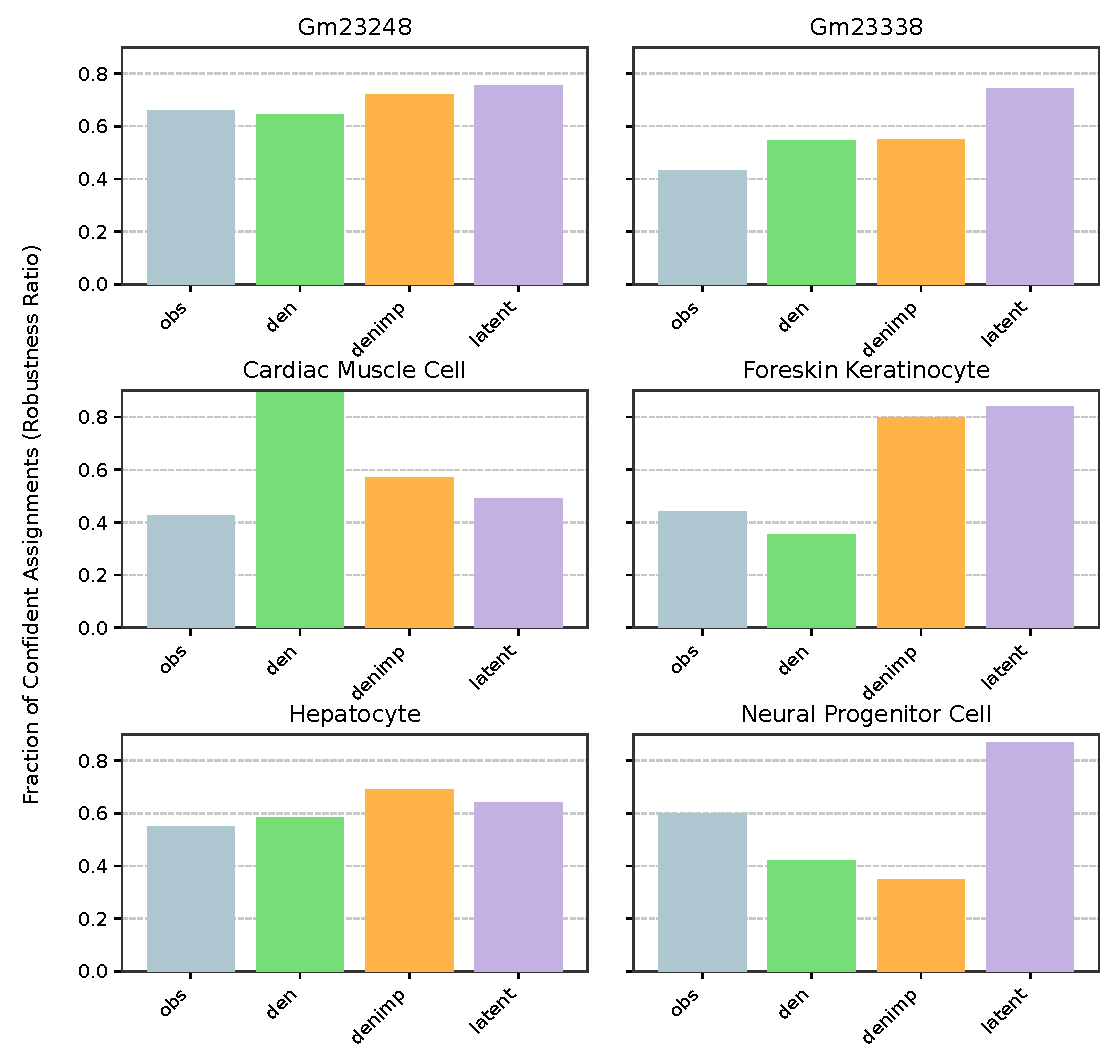
\includegraphics[width=0.62\textwidth]{saga_repro.pdf}
    \caption{\textbf{Chromatin state annotation reproducibility across all six held-out biosamples.} Each panel corresponds to one held-out biosample. Chromatin state annotations were computed from four input sources---observed signals (\emph{obs}), CANDI denoised signals (\emph{den}), CANDI denoised+imputed signals (\emph{denimp}), and CANDI latent embeddings (\emph{latent})---and scored with SAGAconf. Bars show the robustness ratio: the fraction of the genome receiving a confident, reproducible state assignment (higher is more reproducible). In every biosample, at least one CANDI-derived source exceeds the observed-data annotation, with the latent representation most consistently best (highest in four of the six biosamples). Figure~\ref{fig:biol}C shows two representative biosamples from this panel.}
    \label{fig:saga_full}
\end{figure}

\section{Supplementary Methods}

\subsection{Cell Type Merging (Extended ENCODE Dataset)}

To address the sparsity of the $3{,}064 \times 35$ experiment availability matrix while maintaining biological relevance, we implemented a cell type-based merging strategy. This merging strategy significantly improved data density, increasing the median number of available assays per sample from 1 (per biosample) to 6 (per merged cell type). Our merging strategy groups biosamples by their annotated cell type (biosample term name in ENCODE) and further organizes them based on isogenic replicate relationships. Within each cell type, we identify sets of biosamples that are isogenic replicates (derived from the same donor) and share at least three assays in common---these form replicate groups. Each replicate group is assigned a group identifier (grp), and individual biosamples within a group are labeled as replicates (rep). For example, \texttt{cardiac\_muscle\_cell\_grp1\_rep1} and \texttt{cardiac\_muscle\_cell\_grp1\_rep2} represent two isogenic replicates from the same cardiac muscle cell type that share a common set of experiments. Biosamples that lack isogenic replicate annotations or do not share sufficient experiments with other samples are aggregated into a single ``non-replicate'' sample (e.g., \texttt{right\_lobe\_of\_liver\_nonrep}), where experiments are selected to maximize consistency of donor, lab, and biosample accession. This strategy preserves biological relationships while maximizing the number of assays available per merged sample for training.

\subsection{Control Integration and Downsampling}

For each biosample containing ChIP-seq experiments, we obtained the corresponding ChIP-seq control (input) experiments. These control signals are provided as an additional always-available input channel to the model, forming an $(A+1)$-dimensional input where the $(A+1)$-th feature represents the control signal. Controls are never masked during training, serving as a stable reference for batch effect normalization. To simulate varying sequencing depths, we implemented read downsampling in BAM files. The Downsampling Factor (DSF) determines the fraction of reads retained: $\text{DSF} = 1$ retains all reads, $\text{DSF} = 2$ randomly samples 50\% of reads, and $\text{DSF} = 4$ randomly samples 25\% of reads. The default DSF list used during training is $\{1, 2, 4\}$.

\subsection{Output Distributions}

The choice of probability distributions is motivated by the statistical properties of each output type. For raw read counts, we use the negative binomial distribution, which is well-established for modeling sequencing count data due to its ability to capture overdispersion---a common characteristic of epigenomic experiments where variance exceeds the mean. The Poisson distribution is a special case of the negative binomial with fixed dispersion, but empirical studies have shown that epigenomic count data typically exhibit overdispersion, making the negative binomial more appropriate \cite{anders2010differential}.

For processed signal values, we predict $\text{arcsinh}$-transformed $p$-values following previous methods for variance stabilization \cite{hoffman2012unsupervised}. We model these transformed values with a Gaussian distribution, predicting both the mean ($\mu$) and variance ($\sigma^2$). Unlike standard MSE optimization, which implicitly assumes constant variance across all predictions, our approach allows the model to express position-varying uncertainty. By jointly optimizing both parameters via Gaussian negative log-likelihood, the model learns to output higher variance in regions where predictions are inherently more uncertain---capturing aleatoric uncertainty that reflects irreducible noise in the data rather than model limitations.

\subsection{Encoder $\mathcal{E}$}

The encoder integrates epigenomic data $\mathbf{M}$, DNA sequence context $\mathbf{S}$, and experimental covariates $\mathbf{C}_{\text{in}}$ into a latent representation $\mathbf{Z} \in \mathbb{R}^{N \times L' \times d_{\text{model}}}$.

\paragraph{1. Epigenetic Signal Convolution Tower:}
Processes the epigenomic signals with $n_{\text{cnn}} = 3$ depth-wise separable convolution layers. Each layer applies convolution with kernel size $k = 3$, followed by normalization, GELU activation, and average pooling with $\text{pool\_size} = 2$. This progressively reduces the spatial dimension from $L = 1{,}200$ to $L' = 150$ while expanding the feature dimension:
\begin{equation}
    L' = \frac{L}{\text{pool\_size}^{n_{\text{cnn}}}} = \frac{1200}{2^3} = 150
\end{equation}
After each convolution layer, a MetadataCrossAttention module conditions the features on experimental covariates using FiLM (Feature-wise Linear Modulation) \cite{perez2018film}.

\paragraph{2. DNA Sequence Convolution Tower:}
Processes the one-hot encoded DNA sequence with $n_{\text{cnn}} + 2 = 5$ convolution layers. The first three layers use $\text{pool\_size} = 2$, and the final two layers use $\text{pool\_size} = 5$ to match the epigenomic resolution:
\begin{equation}
    L'_{\text{DNA}} = \frac{G}{\text{pool\_size}^{n_{\text{cnn}}} \times 5^2} = \frac{30000}{2^3 \times 25} = 150
\end{equation}
This produces DNA features $\mathbf{S}^{(\text{final})} \in \mathbb{R}^{N \times L' \times d_{\text{model}}}$.

\paragraph{3. Metadata Cross-Attention:}
At each convolutional layer, experimental covariates modulate the learned features through cross-attention. For each assay $a$, we embed the four covariates (depth, run\_type, read\_length, sequencing\_platform) into a query vector $\mathbf{q}_a$. This query attends to the spatial features of that assay, producing scale ($\boldsymbol{\gamma}_a$) and shift ($\boldsymbol{\beta}_a$) parameters for FiLM conditioning:
\begin{equation}
    \mathbf{h}'_a = \boldsymbol{\gamma}_a \odot \mathbf{h}_a + \boldsymbol{\beta}_a
\end{equation}
where $\odot$ denotes element-wise multiplication and $\mathbf{h}_a$ are the features for assay $a$.

\paragraph{4. Fusion:}
The epigenomic and DNA features are concatenated along the feature dimension and projected back to $d_{\text{model}}$ dimensions through a linear layer with layer normalization:
\begin{equation}
    \mathbf{H}^{(0)} = \text{LayerNorm}\left(\mathbf{W}_{\text{fusion}} \left[\mathbf{M}^{(\text{final})}; \mathbf{S}^{(\text{final})}\right] + \mathbf{b}_{\text{fusion}}\right)
\end{equation}

\paragraph{5. Transformer Encoder:}
Applies $n_{\text{sab}} = 4$ transformer encoder layers with $n_{\text{head}} = 9$ attention heads. We use rotary positional embeddings (RoPE) for improved length generalization. Each layer consists of multi-head self-attention followed by a feed-forward network with GELU activation and dropout $= 0.1$:
\begin{align}
    \mathbf{H}^{(i+1)} &= \text{FFN}\left(\text{MultiHeadAttn}\left(\mathbf{H}^{(i)}\right)\right) \\
    \mathbf{Z} &= \mathbf{H}^{(n_{\text{sab}})}
\end{align}

\subsection{Decoders $\mathcal{D}$}

Given latent representation $\mathbf{Z}$ and output covariates $\mathbf{C}_{\text{out}}$, three separate decoders reconstruct the output distributions:

\paragraph{1. Output Covariate Embedding:}
Output covariates are embedded using the same MetadataCrossAttention mechanism as the encoder, providing the model with information about the desired output experimental conditions.

\paragraph{2. Deconvolution Towers:}
Each decoder employs $n_{\text{cnn}} = 3$ transposed convolution layers that invert the encoder's pooling and feature compression. After each deconvolution layer, MetadataCrossAttention conditions the features on output covariates, allowing the model to generate outputs appropriate for specific experimental conditions.

\paragraph{3. Distribution Output Layers:}
\begin{itemize}
    \item \textbf{NegativeBinomialLayer:} Two linear projections produce $\hat{n}$ (via softplus for positivity) and $\hat{p}$ (via sigmoid for $[0,1]$ range):
    \begin{align}
        \hat{n} &= \text{softplus}(\mathbf{W}_n \mathbf{x} + \mathbf{b}_n) \\
        \hat{p} &= \sigma(\mathbf{W}_p \mathbf{x} + \mathbf{b}_p)
    \end{align}

    \item \textbf{GaussianLayer:} Two linear projections produce $\hat{\mu}$ (via softplus) and $\hat{\sigma}^2$ (via softplus):
    \begin{align}
        \hat{\mu} &= \text{softplus}(\mathbf{W}_\mu \mathbf{x} + \mathbf{b}_\mu) \\
        \hat{\sigma}^2 &= \text{softplus}(\mathbf{W}_\sigma \mathbf{x} + \mathbf{b}_\sigma)
    \end{align}

    \item \textbf{PeakLayer:} A linear projection followed by sigmoid produces peak probabilities in $[0,1]$:
    \begin{equation}
        \text{peak} = \sigma(\mathbf{W}_{\text{peak}} \mathbf{x} + \mathbf{b}_{\text{peak}})
    \end{equation}
\end{itemize}

\subsection{Self-Supervised Corruption Strategies}

\paragraph{Full Assay Masking.}
We randomly mask $k$ complete assays for each cell type, where $k \sim \text{Uniform}(1, n_{\text{available}} - 1)$. Both the data AND metadata for selected assays are masked, simulating the imputation scenario where some experiments are entirely missing. At least one assay always remains available per cell type to provide context.

\paragraph{Full Loci Masking.}
We randomly select contiguous chunks of genomic positions (default $\text{chunk\_size} = 40$ positions, $\sim$1kb) and mask these positions across ALL available assays simultaneously. This objective most closely parallels BERT-style masked language modeling, where the model learns to predict masked tokens from surrounding context. Here, genomic positions serve as ``tokens,'' and the model must infer epigenomic signals at masked positions using flanking regions and DNA sequence.

\paragraph{Denoising via Downsampling.}
For assays that remain unmasked, the model is trained to reconstruct the original high-quality signal from potentially downsampled (noisy) observations. The observed regions provide the denoising training signal.

\paragraph{Data Augmentation.}
We apply reverse complement augmentation with probability 0.5. When applied, both the DNA sequence and epigenomic signals are reversed along the genomic axis, and the DNA bases are complemented (A$\leftrightarrow$T, C$\leftrightarrow$G). This data augmentation helps the model learn strand-invariant representations.

\subsection{Training Loci}

We use multiple strategies for selecting training genomic loci:
\begin{itemize}
    \item \textbf{cCRE:} Focus on genomic regions containing candidate cis-regulatory elements, which are enriched with informative epigenomic signals \cite{encode2020expanded}
    \item \textbf{random:} Randomly selected non-overlapping regions across the genome
    \item \textbf{full\_chr:} Complete coverage of specified chromosomes
    \item \textbf{gw (genome-wide):} Full coverage across all autosomes and sex chromosomes
\end{itemize}

For all strategies, we exclude ENCODE blacklist regions (known problematic regions with anomalous signal accumulation) to ensure training data quality. We trained CANDI on 5,000 selected, non-overlapping regions, each spanning 30kb. We excluded chromosome 21, reserving it exclusively for testing purposes. In total, CANDI was trained on 150 million base pairs of genomic sequence, representing approximately 5\% of the human genome.

\subsection{Uncertainty Metrics}

\paragraph{Confidence Calibration.}
To evaluate the reliability of the model's uncertainty estimates, we assess its calibration for all three output types. For counts and signal values, we measure the fraction of observed values that fall within the model's predicted $C\%$ confidence interval for $C \in [0, 1]$. A perfectly calibrated model produces a diagonal line ($y = x$), indicating that $c\%$ of observations fall within the $c\%$ confidence interval.

\paragraph{Concordance Index.}
Beyond interval coverage, we evaluate whether the model's uncertainty estimates correctly rank predictions using the concordance index (C-index). For Gaussian predictions with mean $\mu$ and standard deviation $\sigma$, the C-index measures the probability that the model correctly ranks pairs of observations by their true values. Formally, for a pair of positions $(i, j)$, we compute the probability that observation $i$ exceeds observation $j$ under the model:
\begin{equation}
    P(Y_i > Y_j) = \Phi\left(\frac{\mu_i - \mu_j}{\sqrt{\sigma_i^2 + \sigma_j^2}}\right)
\end{equation}
where $\Phi$ is the standard normal CDF. The C-index is then the AUC-ROC score comparing these predicted probabilities against the true binary labels ($\mathbf{1}[y_i > y_j]$). A C-index of 0.5 indicates random ranking, while 1.0 indicates perfect discrimination. This metric assesses whether the model's distributional predictions meaningfully capture the relative ordering of true signal values.

\subsection{RNA-seq Prediction Details}

For each gene, we extract summary features from epigenomic signals around three key regions: the transcription start site (TSS), gene body, and transcription end site (TES). We use adaptive margins set to 10\% of gene length for TSS and TES regions. From each region, we compute summary statistics including the median, interquartile range, minimum, and maximum signal values. We extract features from four signal sources:
\begin{enumerate}
    \item Observed epigenomic signals from available assays only
    \item Denoised signals for assays where observations were provided as input
    \item Denoised+imputed signals across all 35 assays---combining denoised predictions for available assays with imputed predictions for missing assays
    \item Latent representations $\mathbf{Z}$ extracted from CANDI's transformer encoder
\end{enumerate}

For the latent representations, we compute the same summary statistics across each latent dimension for all three gene regions. We employ nested cross-validation to rigorously evaluate predictive performance while avoiding overfitting. The outer loop uses 5-fold cross-validation to estimate generalization performance, while the inner loop performs hyperparameter selection via grid search with 4-fold cross-validation. Each fold trains a pipeline consisting of standardization, dimensionality reduction (PCA retaining 50--90\% variance), and a regression model. We evaluate ridge and lasso regression, reporting Pearson correlation, Spearman correlation, and $R^2$ between predicted and observed $\log$-transformed TPM values.

\subsection{Chromatin State Annotation Details}

Because CANDI's signal predictions are Gaussian distributions rather than point estimates, we annotate them with a soft-evidence HMM whose emission is the predicted distribution, $b_k(\hat{\mu}_t, \hat{\sigma}^2_t) = P(\hat{\mu}_t, \hat{\sigma}^2_t \mid q_t = k)$, so that predictive uncertainty propagates into the annotation; observed signals and latent embeddings are annotated with a standard Gaussian HMM. We quantify reproducibility with SAGAconf~\cite{shahraki2024robust}, which compares two replicate annotations of a biosample, assigns each genomic position a calibrated reproducibility score, and reports the \emph{robustness ratio}: the fraction of the genome that receives a confident, reproducible state assignment.

\end{document}